\begin{problem}
  {Q1(c)}
  Consider a network $G = (V,E)$ with a source $s$, a sink $t$, and a capacity $c_e$ on every edge $e \in E$.
  Let $A,B$ be a minimum $s-t$ cut with respect to the capacities $c_e$. \\
  Claim: If we add $1$ to every capacity, namely $\forall e \in E, c'_e = c_e + 1 \implies A, B$ is still a minimum $s-t$ cut with respect to $c'_e$ \\
  \textbf{False} \\
  \begin{proof}
  Let $G$ be the graph as pictured below: \\
  \begin{center}
  \begin{tikzpicture}[scale=0.2]
  \tikzstyle{every node}+=[inner sep=0pt]
  \draw [black] (10.3,-24.6) circle (3);
  \draw (10.3,-24.6) node {$s$};
  \draw [black] (20.6,-32.9) circle (3);
  \draw (20.6,-32.9) node {$b$};
  \draw [black] (20.6,-16) circle (3);
  \draw (20.6,-16) node {$a$};
  \draw [black] (31.3,-24.6) circle (3);
  \draw (31.3,-24.6) node {$c$};
  \draw [black] (47.6,-24.6) circle (3);
  \draw (47.6,-24.6) node {$t$};
  \draw [black] (12.64,-26.48) -- (18.26,-31.02);
  \fill [black] (18.26,-31.02) -- (17.95,-30.13) -- (17.33,-30.9);
  \draw (14.44,-29.24) node [below] {$1$};
  \draw [black] (12.6,-22.68) -- (18.3,-17.92);
  \fill [black] (18.3,-17.92) -- (17.36,-18.05) -- (18,-18.82);
  \draw (14.44,-19.81) node [above] {$1$};
  \draw [black] (22.97,-31.06) -- (28.93,-26.44);
  \fill [black] (28.93,-26.44) -- (27.99,-26.53) -- (28.6,-27.32);
  \draw (26.96,-29.25) node [below] {$1$};
  \draw [black] (22.94,-17.88) -- (28.96,-22.72);
  \fill [black] (28.96,-22.72) -- (28.65,-21.83) -- (28.02,-22.61);
  \draw (24.94,-20.79) node [below] {$1$};
  \draw [black] (34.3,-24.6) -- (44.6,-24.6);
  \fill [black] (44.6,-24.6) -- (43.8,-24.1) -- (43.8,-25.1);
  \draw (39.45,-25.1) node [below] {$2$};
  \end{tikzpicture}
  \end{center}
  Note that a min cut in $G$ is $A = \{s, a, b\}, B = \{c, t\}$ with a value of $2$ \\
  Now consider $G'$ \\
  \begin{center}
  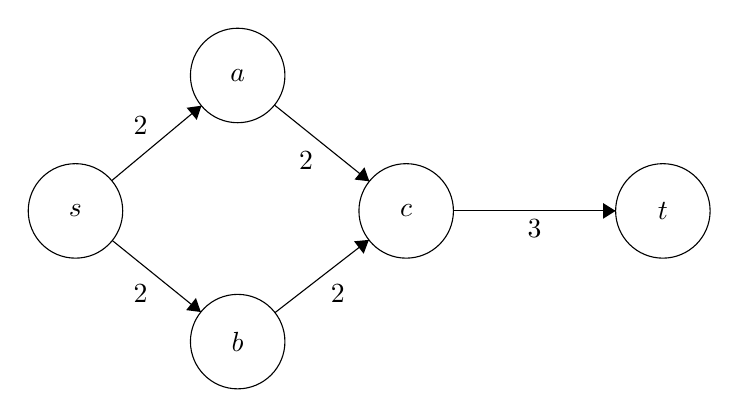
\begin{tikzpicture}[scale=0.2]
  \tikzstyle{every node}+=[inner sep=0pt]
  \draw [black] (10.3,-24.6) circle (3);
  \draw (10.3,-24.6) node {$s$};
  \draw [black] (20.6,-32.9) circle (3);
  \draw (20.6,-32.9) node {$b$};
  \draw [black] (20.6,-16) circle (3);
  \draw (20.6,-16) node {$a$};
  \draw [black] (31.3,-24.6) circle (3);
  \draw (31.3,-24.6) node {$c$};
  \draw [black] (47.6,-24.6) circle (3);
  \draw (47.6,-24.6) node {$t$};
  \draw [black] (12.64,-26.48) -- (18.26,-31.02);
  \fill [black] (18.26,-31.02) -- (17.95,-30.13) -- (17.33,-30.9);
  \draw (14.44,-29.24) node [below] {$2$};
  \draw [black] (12.6,-22.68) -- (18.3,-17.92);
  \fill [black] (18.3,-17.92) -- (17.36,-18.05) -- (18,-18.82);
  \draw (14.44,-19.81) node [above] {$2$};
  \draw [black] (22.97,-31.06) -- (28.93,-26.44);
  \fill [black] (28.93,-26.44) -- (27.99,-26.53) -- (28.6,-27.32);
  \draw (26.96,-29.25) node [below] {$2$};
  \draw [black] (22.94,-17.88) -- (28.96,-22.72);
  \fill [black] (28.96,-22.72) -- (28.65,-21.83) -- (28.02,-22.61);
  \draw (24.94,-20.79) node [below] {$2$};
  \draw [black] (34.3,-24.6) -- (44.6,-24.6);
  \fill [black] (44.6,-24.6) -- (43.8,-24.1) -- (43.8,-25.1);
  \draw (39.45,-25.1) node [below] {$3$};
  \end{tikzpicture}
  \end{center}
  Note that the cut $A = \{s, a, b\}, B = \{c, t\}$ now has a value of $4$, whereas the cut $A' = \{s, a, b, c\}, B' = \{t\}$ has a value of $3$ \\
  \end{proof}
\end{problem}
